\chapter{Apartado A}
\label{chapter:tarea_a}

El objetivo del \textit{Apartado A} es conseguir los parámetros intrínsecos y extrínsecos de las cámaras situadas a la derecha e izquierda de un sistema estereoscópico. En la Figura \ref{fig:stereo_camera} se muestra un ejemplo de cámara estereoscópica \footnote{ \href{https://commons.wikimedia.org/w/index.php?curid=8076697}{De John Alan Elson - http://www.3dham.com/, CC BY-SA 4.0, } https://commons.wikimedia.org/w/index.php?curid=8076697} (no digital). Con estos parámetros se obtiene un modelo de cámara para cada subsistema.

\begin{figure}[h]
    \centering
    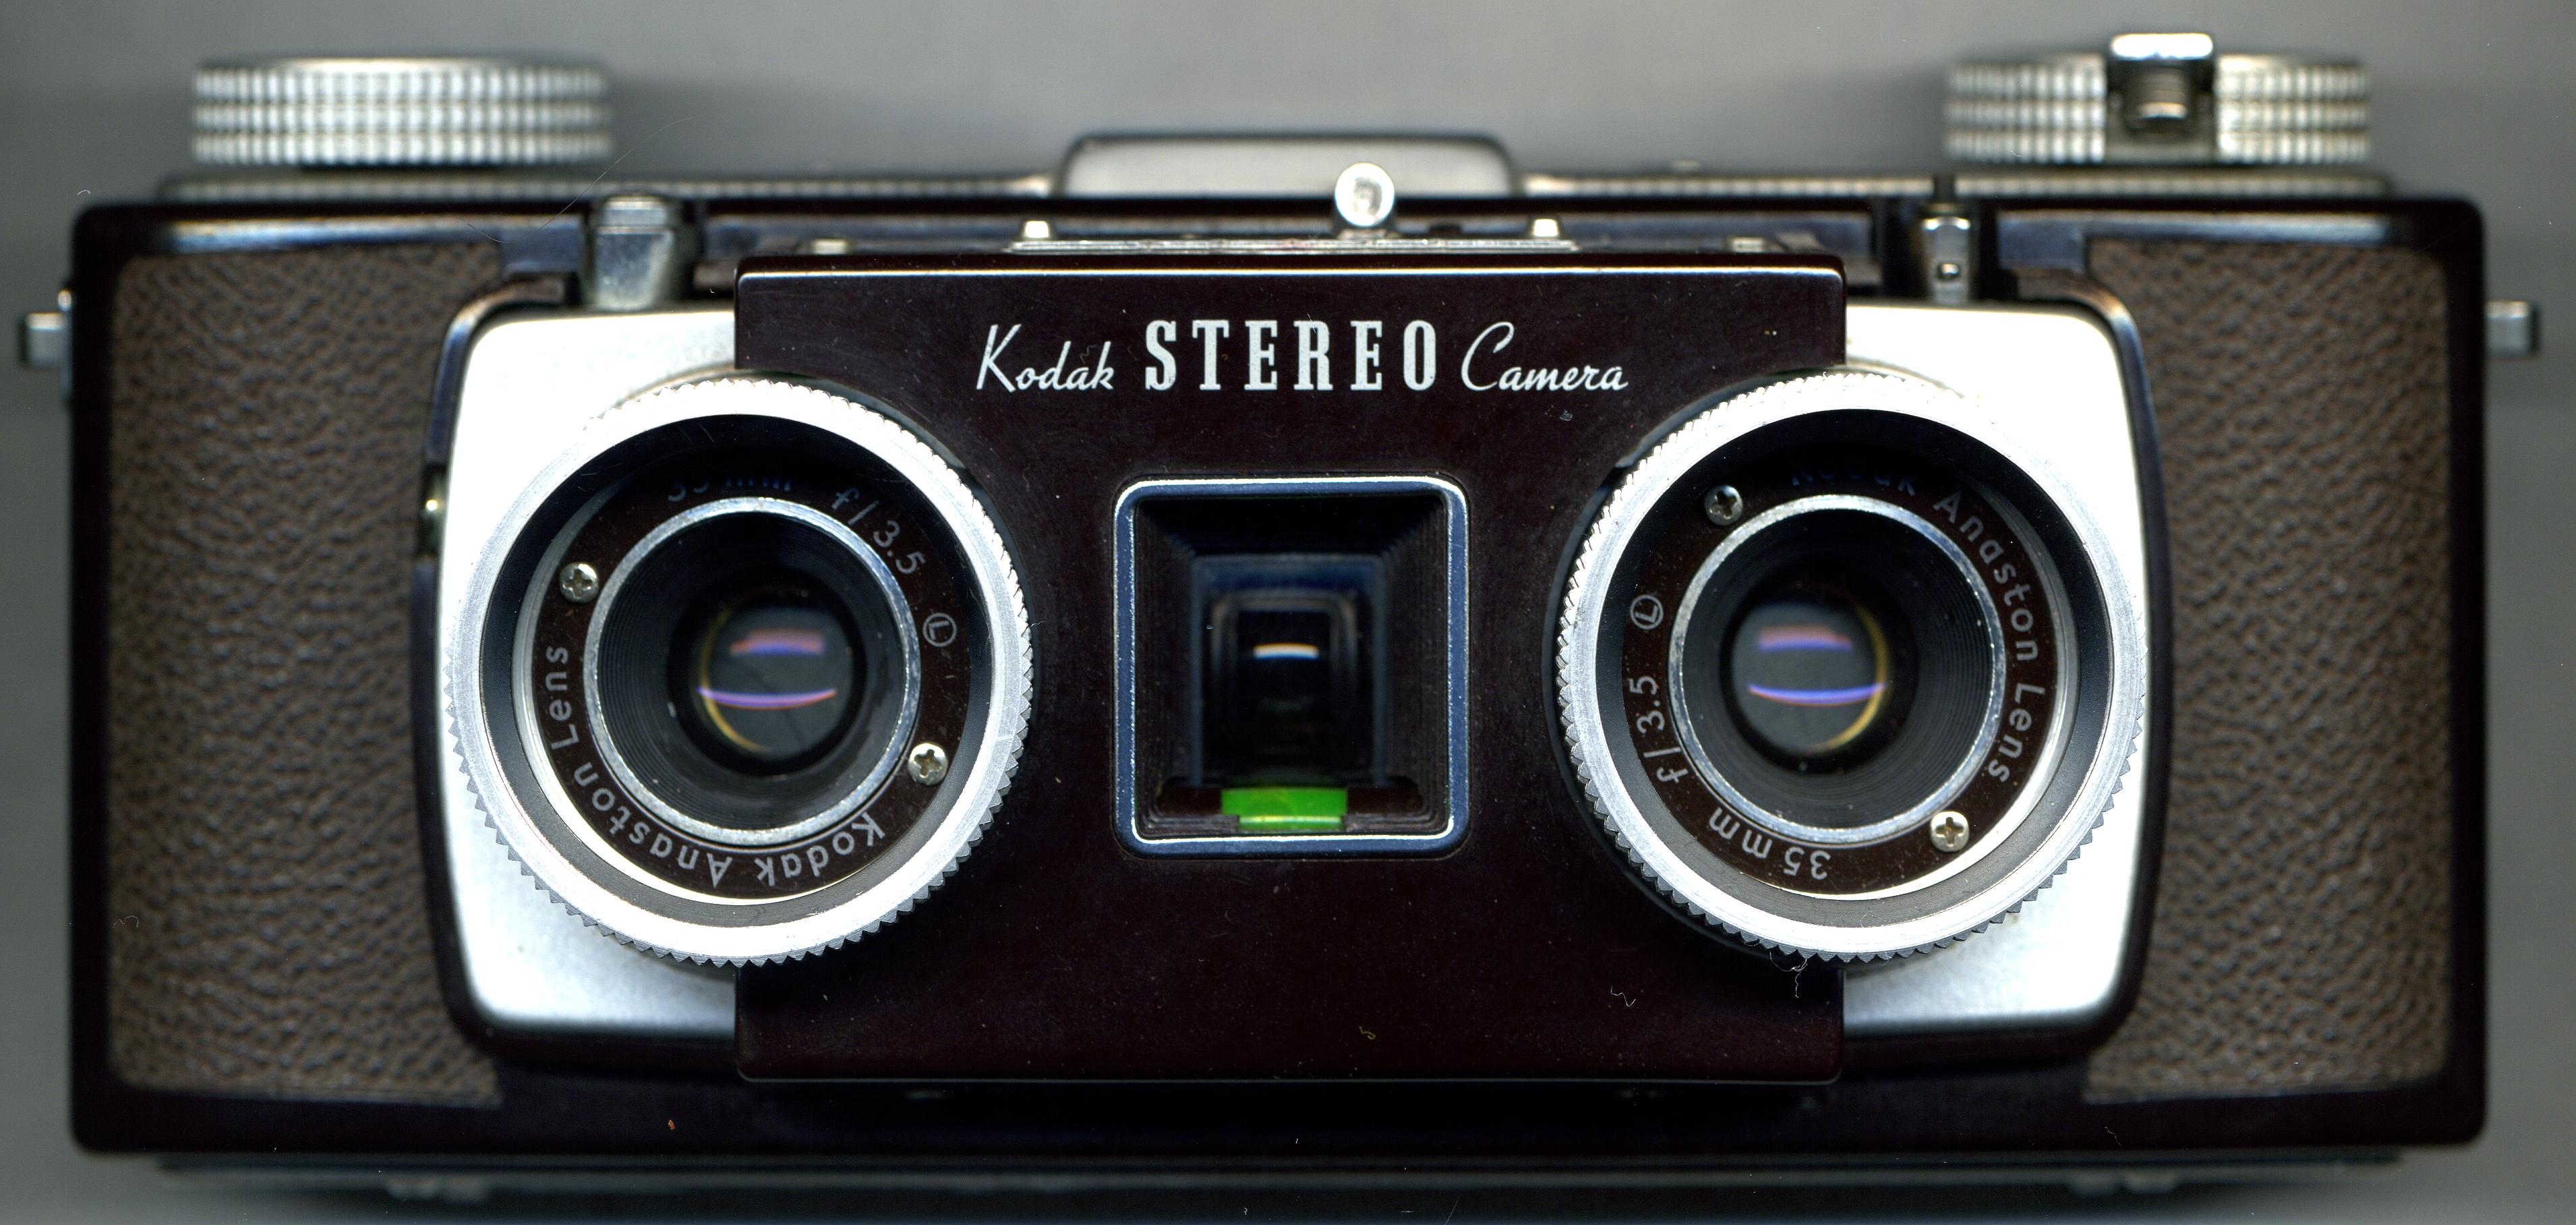
\includegraphics[width=0.5\textwidth]{Lab_1/template/figures/stereo_camera.jpg}
    \caption{Cámara estereoscópica.}
    \label{fig:stereo_camera}
\end{figure}

En este apartado trabajará con el notebook y las imágenes de las carpetas \textit{right} y \textit{left}. En primer lugar, fíjese en la documentación de OpenCV del método \texttt{cv2.calibrateCamera()} \footnote{Doc. \href{https://docs.opencv.org/4.x/d9/d0c/group\_\_calib3d.html\#ga687a1ab946686f0d85ae0363b5af1d7b}{cv2.calibrateCamera()} https://docs.opencv.org/4.x/d9/d0c/group\_\_calib3d.html\#ga687a1ab946686f0d85ae0363b5af1d7b}. Intente detectar los argumentos que requiere este método y cómo podrían derivarse de las imágenes. 

Una vez hecho ese ejercicio mental, deberá seguir los pasos de este enunciado para conseguir un modelo de cámara a partir de las imágenes de cada carpeta:



\section*{Tarea A.1: Carga de Imágenes}
\addcontentsline{toc}{section}{Tarea A.1: Carga de Imágenes}
Defina y ejecute el método para cargar imágenes \texttt{load\_images()}. Deberá pasar una lista que contenga las rutas de todas las imágenes de la carpeta \textit{left}.

\section*{Tarea A.2: Detección de Esquinas}
\addcontentsline{toc}{section}{Tarea A.2: Detección de Esquinas}
Detecte las esquinas de los patrones usando \texttt{cv2.findChessboardCorners()}. Refine las detecciones con \texttt{cv2.cornerSubPix()}.

\textbf{Detección.} La función \texttt{cv2.findChessboardCorners()} de OpenCV busca el patrón de calibración en cada imagen y devuelve una tupla con dos elementos. El primer elemento es \texttt{False} si la detección del patrón falla y \texttt{True} si tiene éxito. El segundo elemento contiene las coordenadas de las esquinas del patrón, que solo son válidas si la detección fue exitosa (es decir, si el primer elemento de la tupla es \texttt{True}). Tenga en cuenta que los resultados de la llamada a esta función se almacenan en una lista, de manera que el elemento $i$ de esa lista corresponde al resultado de procesar la imagen $i$ cargada previamente.

\textbf{Refinamiento.} Se utiliza la función \texttt{cv2.cornerSubPix()} para refinar las detecciones de las esquinas. Tenga en cuenta que esta función necesita las imágenes de entrada en escala de grises.

\textbf{Nota:} Inspeccione las imágenes de forma manual y compruebe que el patrón está formado por 8 filas y 6 columnas de esquinas.


\section*{Tarea A.3: Comprobación de Detecciones}
\addcontentsline{toc}{section}{Tarea A.3: Comprobación de Detecciones}
Compruebe que las detecciones anteriores (tanto las iniciales como las refinadas) son correctas dibujando los resultados con \texttt{cv2.drawChessboardCorners()}.

Dibuje en las imágenes los puntos detectados por \texttt{cv2.findChessboardCorners()}. Por razones de eficiencia, la función utilizada modifica directamente las imágenes pasadas por parámetro en lugar de hacer una copia. Para evitar perder las imágenes originales, es mejor hacer una copia de ellas de antemano. Utilice la copia para realizar el ejercicio.

Una vez dibujadas las detecciones, deberá diseñar una función de visualización de imágenes con OpenCV. Para ello, podrá apoyarse en los métodos \texttt{cv2.imshow()}, \texttt{cv2.waitKey()} y \texttt{cv2.imwrite()}.


\section*{Tarea A.4: Obtención de Coordenadas 3D de las Esquinas del Patrón}
\addcontentsline{toc}{section}{Tarea A.4: Obtención de Coordenadas 3D de las Esquinas del Patrón}
Defina y ejecute el método \texttt{get\_chessboard\_points(chessboard\_shape, dx, dy)} que proporcione las coordenadas 3D de las esquinas del patrón.

Para ello, el punto de coordenadas $[0, 0, 0]^\top$ es la primera esquina detectada en el patrón de calibración. El eje X corresponde al lado corto del patrón, mientras que el eje Y corresponde al lado largo. La función devolverá un array de \texttt{numpy} de tamaño $ N \times 3 $ que contenga las coordenadas $(x, y, z)$, donde N es el número de esquinas.

Para diseñar la función, tenga en cuenta que \texttt{chessboard\_shape} es una tupla que contiene el número de esquinas por fila y columna del patrón. Por otro lado, \texttt{dx} y \texttt{dy} corresponden al ancho y alto de cada cuadrado del patrón de calibración, que en esta práctica es de $30mm$.

Tenga en cuenta que deberá proporcionar una lista que contenga los puntos para todas las imágenes con detecciones correctas.


\section*{Tarea A.5: Calibración de la Cámara Izquierda}
\addcontentsline{toc}{section}{Tarea A.5: Calibración de la Cámara Izquierda}
Utilice \texttt{cv2.calibrateCamera()} para obtener los parámetros de calibración para la cámara situada a la izquierda.

Deberá utilizar los resultados de \texttt{cv2.findChessboardCorners()} y el conjunto de puntos obtenido con \texttt{get\_chessboard\_points()} del ejercicio anterior.

Filtre aquellas detecciones de esquinas que hayan sido procesadas correctamente. Recuerde que \texttt{cv2.findChessboardCorners()} devuelve una tupla donde el primer elemento es un Booleano. Este elemento indica si la detección es correcta o no.


\newpage
\section*{Preguntas}
\addcontentsline{toc}{section}{Preguntas}

\vspace{5mm}
\begin{tcolorbox}[colback=gray!10, colframe=gray!30, coltitle=black, title=Pregunta A.1, halign=left]
Repita el proceso (carga de imágenes, detección, comprobación de esquinas, etc.) para la cámara situada a la derecha. Deberá adjuntar:
\begin{itemize}
    \item Al menos 2 imágenes con la detección de esquinas.
    \item Los parámetros intrínsecos y extrínsecos de la cámara.
    \item Los coeficientes de distorsión y el error de calibración.
\end{itemize}
\end{tcolorbox}


\vspace{5mm}
\begin{tcolorbox}[colback=gray!10, colframe=gray!30, coltitle=black, title=Pregunta A.2, halign=left]
¿Observa diferencias entre las detecciones de esquinas realizadas con \texttt{cv2.findChessboardCorners()} y las refinadas con \texttt{cv2.cornerSubPix()}? Apoye su respuesta adjuntando imágenes.
\end{tcolorbox}

\vspace{5mm}
\begin{tcolorbox}[colback=gray!10, colframe=gray!30, coltitle=black, title=Pregunta A.3, halign=left]
Por ahora, ha asumido que el número de imágenes que le hemos ofrecido es adecuado para obtener una calibración adecuada. Sin embargo, en su proyecto final, ¿cuántas imágenes cree que debería tomar con su cámara para calibrarla? Responda a esta pregunta y obtenga un orden de magnitud dibujando un diagrama de Pareto. En este, aparecerá el número de imágenes consideradas (eje horizontal) vs. el error de calibración (eje vertical).
\end{tcolorbox}